\documentclass[10pt]{article}
\usepackage{fullpage, graphicx, url}
\setlength{\parskip}{1ex}
\setlength{\parindent}{0ex}
\title{3Depict User Manual}

\usepackage{wrapfig}

\begin{document}
\title{3Depict - Valued point cloud visualisation and analysis}

\section{3Depict Basics}
\subsection{Introduction}


  3Depict is an open source computer program designed for the analysis of point clouds. The program is designed around interactive data analysis, with a view to combine the rapid feedback, ease of use and flexibility in a single system.  
 3Depict is designed purely for post-processing of 3D point data, and was originally primarily targeted to users of Atom Probe Tomography. Other users may find the program useful, and are encouraged to seek assistance. 
 
\subsubsection{Background}


  3Depict attempts to fill a perceived need for freely available flexible point data visualisation. This program is designed to manipulate and modify point data in a way which the author has otherwise not found a suitable program to do.  
 With this program, point data can be visualised using a fully implemented camera system, edited with directly interactive objects, and subjected to various analysis algorithms. A real-time plotting system is also provided to generate analyses of your data on the fly. External programs can be engauged as part of the system to create new analyses that ``clip into'' the analysis. 
 
\subsubsection{What is Open Source?}
\begin{wrapfigure}{r}{0.7\textwidth}
 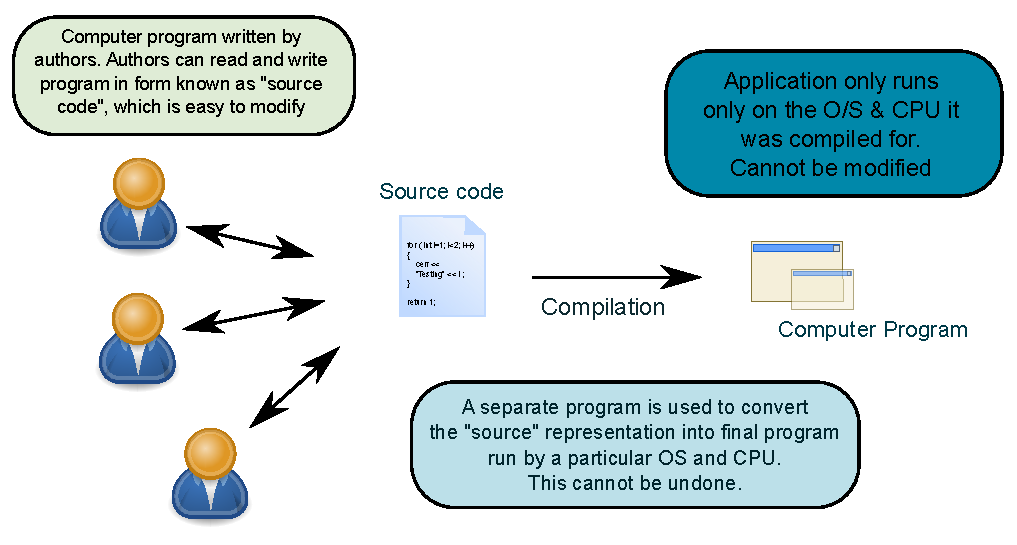
\includegraphics[width=0.7 \textwidth,keepaspectratio=true]{./figures/compilation.pdf}
 % camera.pdf: 578x382 pixel, 72dpi, 20.39x13.48 cm, bb=0 0 578 382
 \caption{Closed-source programs only provide the final application, are neither human readable nor modifiable, and will only work on a specific platform. By contrast open source programs distribute the source-code as well as the application. The source code is the core logic which can be made to work on many platforms due to the invariance of the program logic.}
 \label{fig:compilation}
\end{wrapfigure}
Open source programs are programs which distribute not only the executable code, which is understood by the computer (so called machine code), but also provides the version of the program as it was written by humans as well. This provides external users with the possibility of either by themselves, or by engaging a third party. With the source code one can verify the correctness of the system, alter behaviour or otherwise modify the program, or even reuse sub-sections of the program elsewhere. 

Modifications to the program itself may include migrating the program to newer or older systems, adding new functionality, or correcting errors in the program implementation.  
 
To provide the user with these capabilities, the program is distributed with a so-called ``free'' copyright licence. The program is distributed at no cost to the end user, and the copyright attached to the program explicitly allows modification and re-distribution (copying) of the program to other parties, without requiring the author's consent.  

Note that there are restrictions on what may be done with the program, for example it is in violation of the licence to claim ownership of the program, or to use technical measures to prevent access to the program, or modification thereof. The licence used in the program is a generic one shared by many free (as in freedom) software programs  

If you have been charged for this program, it is suggested that you request a refund and obtain a free copy from the main website. If you wish to have the full licence details (GNU General Public Licence Version 3), please see the COPYING file distributed with this program. If this is not available, please see the project website, or perform an internet search for the licence name. 
\subsubsection{Who wrote this program?}


This program was writen by D. Haley, in his spare time. A. Ceguerra provided assistance with debugging and fixing the Macintosh version, and providing executable versions of the program for OSX. 
\subsubsection{Getting help}


Assistance with this program may be freely obtained over the internet at \url{http://threedepict.sourceforge.net}. Questions regarding use of the program, feature or bug reports will be attended to as soon as possible. 
\subsubsection{Alternate documentation}
For the more visually inclined, screencasts of the program have been created, and are available on the project website. 

\subsection{ Getting started }
\subsubsection{ Requirements}


The minimum requirements for running 3Depict are not known. The author wrote a substantial portion of the program on a machine with a 4 and 12 Gigabyte drives, and a 1.6GHz processor, which normally runs at 800MHz and 1 GB of ram.  

Whilst a newer machine may run the program faster, intelligent use of the filter system may allow for complex analyses even on low-end machines. Every effort is expended by the author to ensure that the program can be run on as many devices as possible; if your platform is not supported, it may be possible for either you, or the author to generate executables for your system. See the section ``Getting Help'' for contact details.  

If you are experiencing video card problems, first ensure that other 3D programs do not experience the same problems. Otherwise, please contact the author for assistance -- there should be no requirement for vendor-specific hardware. 

\subsubsection{Platform specific notes}
Note that whilst every effort is made to ensure that the program will run on a variety of systems, small system-specific quirks may be evident, particularly on platforms to which the authors do not use regularly (e.g. windows). Secondly, due to slight differences between platforms some functions may be remapped to other mouse/key combinations.  
Linux: No notes Mac: CTRL keys may sometimes be mapped to the Command key. Windows: A current outstanding bug is a visible ``flicker'' when interacting with the plot view.  
\subsubsection{Licence}
This program is distributed under the GNU General Public Licence Version 3 (GPLV3). Information on the copyright of this program is available under the COPYING file in the program directory. The following pre-amble is included here:  
 
\subsubsection{Installing the program}
The installation method for the program depends upon your chosen operating system. The most-up-to-date notes are available on the project website.  

\subsection{Understanding the interface}

The program interface consists of three different views. On the left, there is the data, cameras and tools panels, with are used to generate data for visualisation, and to provide an interface into changing properties in a structured manner. On the right, the view is split into two sections; at the top, there is the 3D view. At the bottom are the plotting, raw data and console output panels.  

Each panel may be hidden, either by double clicking the ``sash'' between the two windows, by selecting the respective item from the view menu or by its keyboard shortcut key.  

At the very bottom of the program, a status bar is shown -- here messages are shown to provide hints on how to use the program, or to communicate information relating to the program's internal state. 
\subsubsection{The 3D View}
\begin{wrapfigure}{r}{0.65\textwidth}
 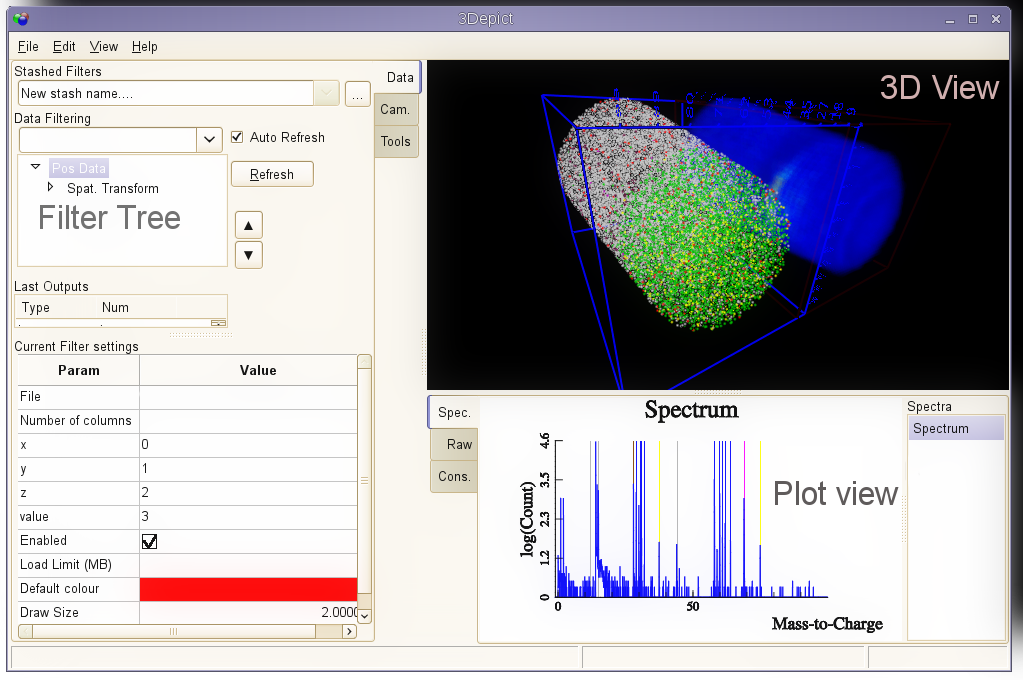
\includegraphics[width=0.65 \textwidth,keepaspectratio=true]{./figures/interface.png}
 % camera.pdf: 578x382 pixel, 72dpi, 20.39x13.48 cm, bb=0 0 578 382

 \caption{Interface layout. The 3D view, plot panel and filter tree are labelled.}
 \label{fig:interfaceLayout}
\end{wrapfigure}
The 3D view is used to show the three-dimensional objects generated during a data analysis, and provides a direct method of interaction with the 3D Scene. Through the use of the mouse (or other pointing device), the 3D view can be manipulated to change the view position and orientations. Some objects in the 3D view are interactive, and will be indicated by an overlay in the top right of the window when the pointer is on top of such an object. 


\subsubsection{Basic movement}
\begin{wrapfigure}{r}{0.45\textwidth}

 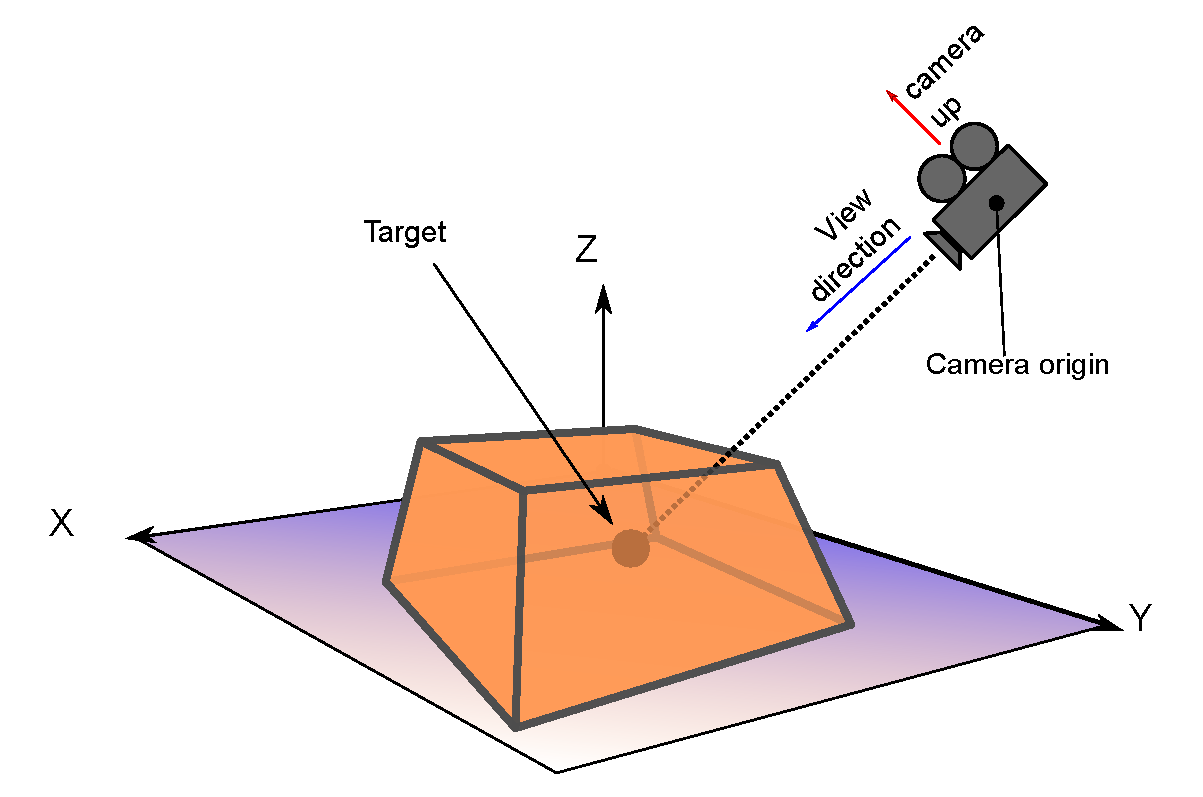
\includegraphics[width=0.45 \textwidth,keepaspectratio=true]{./figures/camera.pdf}
 % camera.pdf: 578x382 pixel, 72dpi, 20.39x13.48 cm, bb=0 0 578 382

 \caption{Basic camera layout. Each camera has a position, an up direction and a target. The 3D view is as seen by the camera. Cameras may be saved and recalled to return to specific views.}
 \label{fig:camera-basics}
\end{wrapfigure}
The 3D view represents your camera into a 3D scene of your construction; it is by manipulation of cameras that the view is interacted with; so you may zoom, orbit, pan, roll or swivel the camera view. If you are lost at any time, you may reset the view by tapping the space bar. To change the axis along which the view is reset, hold the CTRL or SHIFT buttons whilst resetting.  

The basic 3D view consists of a ``target'' based camera, so when you move the camera, the camera will orbit around this target. To interact with a scene, hold down the left mouse button and move the mouse to control the camera.  


The basic keys for controlling the camera move mode are :  
\begin{itemize}
\item  NONE: Orbit camera 
\item CTRL: Pan camera 
\item  TAB : Swivel camera (Look about)
\item  CTRL +TAB : roll camera around viewport centre. Note that the rolling motion is controlled by the position of the mouse click.

\end{itemize}
 For any motion, the SHIFT key may be used to increase the camera move speed. 
\subsubsection{Creating a scene}


Initially the program window will appear blank. To provide a more interesting view, it is necessary to inject data into the program.  To do so, select the File menu, and then select using ``Open''. At time of writing, only two formats are currently supported. Firstly are ``POS'' files, which consist of X,Y,Z and a value (usually mass-to-charge) records, these are repeated across the file. The technical description of these files is fixed-width-records of IEEE594 32 bit floating point in big-endian (PPC) byte order, totalling 16 bytes for each (X,Y,Z,V) record.  

To load a file, navigate to an existing POS file on your disk. If you do not have a POS file, small example files are available on the project website.  

Upon selecting the file and then OPEN/OK, the file will be loaded into the viewport. Note that the entire file is not loaded, but rather a random selection of elements in the file. It is recommended that for performing analyses, any analyses are initially conducted with this small random sub-selection, and then the entire dataset can be loaded when the analysis ``tree'' is ready. 
\subsubsection{The analysis tree}


Loading this file populates a small treeview on the data pane (at the left). This tree is referred to as the ``analysis'' tree, and each item in the tree is called a ``filter''. The tree is responsible for producing the output data in the scene, and a good understanding of the behaviour of this tree is required to extract the maximum benefit from the program.  
 
To modify the tree, you may add new or remove existing components of the tree. Changes to the tree may be undone using the ``Edit'' menu, or with the keyboard shortcut Ctrl-Z.  

Note that with every modification of the tree, the 3D scene and any plots will be recomputed. The time of computation is dependent upon the amount of data that is to be analysed, and can be reduced through sampling or volume restriction methods. 
\subsubsection{Basic manipulation}


Initially the tree will be empty, and contain no items. To add a base to the tree, a file must be loaded, which will add a ``base'' element. This will initially be ``collapsed'' so that only the first element is visible. To expand the tree, either select the symbol to the left of the tree view (+ or $>$). Clicking this again will collapse this section of the tree. This allows for the viewing of only the component that is actively being worked on  

To delete an item, simply select the item to delete with the mouse, and then use either the ``DELETE'' or ``BACKSPACE'' keys on your keyboard. Note that clicking on an already selected item will activate the name edit mode. To exit this mode, press ESCAPE. 
\subsubsection{Adding new items}


New items can be added to the tree by selecting the filter to add from the dropdown box immediately above the tree. When selecting a new filter to add; an element in the tree must be selected, where the new filter will be placed. If there is no item selected, an error will be shown in the status bar.  

Once an item is added, the filter tree is thus modified and a recomputation of the scene will occur. Approximate progress on the filter update is visible in the status bar. During an update, only limited interaction with the program is permitted. An update may be cancelled at any time with the ESCAPE key. 

\subsubsection{Plots}
The available plots are listed on the right hand side of the plot view panel. YOu can select the active plot from the list. The ites in the list take their name from the filter from which they originates name (there are exceptions to this rule, i.e. composition profiles). Several plots may be drawn at once by holding down the CTRL key when selecting the plot to draw from the plot list box. \subsection{The analysis}
\subsubsection{Tree view}
\subsubsection{Understanding the tree}
The tree is a flexible and powerful system for constructing your own analyses, after some use this will become a familiar and readily modifiable system for performing your analyses, however the initial structure of the program may take some getting used to. If you are familiar with programs such as \emph{Paraview}, you may already be familiar with this concept.  

The filter tree essentially is a system for injection, manipulation and display of the data in the program. The tree becomes an ``assembly line'' for the view of data in the 3D and plot views. Data may be considered to propagate from the ``base'' of the tree downwards, with each filter in a direct line somehow modifying the data from above in some way.  

When data reaches the end of the filter tree it is ``picked up'' by the 3D,plot or console panels, depending upon the nature of the data. Each node in the tree may be considered in what is called a ``parent-child'' relationship. Each element in the tree (except the first) has a ``parent'', and thus may have their own ``child'' elements. Each ``parent'' may, in fact, have many children.  

The basic method for data flow is that a parent gives a copy of the data it has processed to its ``children'' to modify in some way. Each ``child'' has its own copy\footnote{Technical note: the ``copy'' system is at the discretion of each filter. Child filters are given a reference to the parent data which restricts modification of the parent's data by the children; children may or may not duplicate this data, propagate or terminate the reference.}{of the data from the parent, which it modifes. In turn this child then gives a copy of the data to each of its own children. If a filter has no children it then passes the data to either the 3D view, the plot view or the console view, depending upon the data type.  
 Using this method, one may create a variety of different analyses; for example, one may wish to subsample data before performing a time-consuming spatial analysis, or one may wish to clip the data to remove unwanted sections before generation of a mass spectrum. The flexibility of the filter system supports this concept.it is not the object that moves, but it is rather yourself  

\subsubsection{Editing the tree}

Note that items in the filter tree can be moved. You may move any filter to a new parent, to copy instead of moving, hold down the CTRL (under mac use the APPLE key) whilst moving to duplicate the filter, rather than moving it.  

You may also rename filters in the tree; The filter name may be used by the filter to generate its output, e.g. spectrum plots will take the plot title from the filter name. 


 To fully understand the camera model, it is necessary to understand the parameters in the camera property tab. One can select the position of the camera, a position that the camera is always looking at (look-at mode), the camera ``up'' direction, and the field of view.  

 With the exception of the field of view, these parameters are dynamically modified when interacting with the 3D scene (see section X). The camera field of view, however requires special mention. The field of view of the camera is the angle that the camera look at. Human vision is around 120*, and is much narrower for suffers of tunnel vision (say, 30*). A bird has a full 360 degree field of view (it can see in all directions without needing to turn its head). By default the camera is set to 90*. To get the ``fish-bowl'' effect, where close obects appear very large, this number can be increased. To get an effective orthogonal camera, this number can be set very low. Note that changing this value will also have the apparent effect of zooming the camera in or out, so tapping SPACE to reset the camera view is recommended for large changes. 
\subsubsection{Tools panel}


  The tools panel offers several options on changes to the way the program operates internally. \begin{itemize}
\item  Smooth and Translucent objects: This enables so-called ``alpha blending'' in the 3D scene, where appropriate which allows for non-opaque objects, and anti-aliased objects. This mode alters the way in which objects are rendered in the 3D scene and is in effect a quality-apperance tradeoff. Most of the time you will probably want it set to ON. The program may render the 3D scene slightly faster if this is disabled.
 
\item  Enable lighting : 3D objects do not look very 3D if you are only seeing them on a 2D screen. Computer graphics works around this by simulating the effect of having a 3D lighting source. This might provide minor performance improvements if disabled, at the cost of clarity of rendering.
 
\item Enable filter caching: This alters the way in which the program processes the filter tree. Normally, the program performs what is known as a depth-first search, and propagates data generated by the program from one filter to the other. Intermediate copies are kept by the filters themeselves to speed up recomputation. However, this strategy has a large downside, which is memory consumption. Disabling this will reduce memory consumption by filters, but will mean that any change to the filter tree, no matter how small, will cause the entire tree to be recomputed, including data loading.

\end{itemize}

\subsubsection{Stashes}

Instead of enabling or disabling sections of the tree, the program supports ``stashes'' as a place to put sections of the analysis tree for later use without using them in the analysis section. To create a ``stash'', select a section of the filter tree to ``stash'', then in the ``stashed filters'' dropdown on the data tab, type the name of the stash you wish to create (this is up to you), and press enter. Once done, a duplication of the subtree specified (ie all the filters below the selected one, and the selected one too), is made. You can view the contents of the stash by selecting the button next to the stash dropdown, and you may delete stashes however you cannot edit them.  

To use a stash, select a filter in the tree and then click the dropdown button on the stash combo box, and then select the stash you wish to use. This will place the stash as a child of the selected filter. Note that the stash can be used multiple times.  

\subsubsection{Plots}
 Several plots may be drawn at once by holding down the CTRL key when selecting the plot to draw from the plot list box.  
\subsubsection{Miscellaneous features}
\subsubsection{Save}
 The current programs state can be saved to an ``XML'' state file for later analysis. Note that this file cannot be copied freely between computers, as the data is not kept inside this file, only a reference to the file on your drive. Fortunately, this file can be easily edited by hand using programs such as ``wordpad'' (windows), ``textpad'' (mac), or any reasonable text editor (all platforms).  
 The program state may be restored by opening an external file. Note that opening an existing program state file will erase your current state. If you wish to merge the two states together into a single analysis, use the ``merge'' option.  
\subsubsection{Undo}
 The program has an undo feature which can be used to abort the last changes to the filter tree. Note that for memory reasons, the results of the computation are not stored, and will need to be recomputed.  
\subsubsection{Raw Data}
 The raw data pane may be used to obtain the raw XY data used to generate the plots. This can either by copied and pasted, or alternately saved to file.  
\subsubsection{Export Menu}
 Plots, images and ion data may be exported from the program. The output formats for 3D images is ``Portable Network Graphic (PNG)'' images; these are supported by almost all image viewers. 

For plots, you may save in either (Scalable Vector Graphic (SVG)) or ``PNG'' forms. Note that due to the nature of the SVG files, no resolution is needed, and the image can be reproduced at any scale. Furthermore the SVG can be used later to generate PNG images at the required size for output (I recommend the program ``inkscape''). Alternately saving as PNG can be done, and you will be prompted for the desired image size.

 Exporting Ion Data can be done in several ways; you may export only the visible ions, or alternately, you may export only a subset (for example one or two ranges) of the data, depending upon the filter that the data originated from. The output format will be in Big-endian ``POS'' format.  
\subsubsection{Autosave}
 The program will generate an autosave file periodically. If the program crashes, it will look for an autosave file and prompt you to restore it. Note that only the program settings are saved, not the data, so recomputation will be neccesary.  

\section{Data model}
\subsection{Data Types}
Different data can propagate through the filtering system before it is seen in the 3D view. The currently available types are ion, range and plot types. Although these are used internally by the program, understanding the type system may enable more advanced use of the program. If you are not interested in this, skip to the next section.  

Ions Each ion represents a point in space, which has a value type associated with the point. For example, one might consider a point in a dataset where positions represent atomic positions, and the value is the measured atomic mass. Ions are grouped together by different filters, and each group may be represented with a unique colour and size.  

\subsubsection{Range}
This is a special datatype which propagates information through the filter tree. The data represents non-overlapping regions of the value space which are to be tagged as belonging to a certain group. This data type has now actual output into the 3D scene, but can alter the manner in which ``downstream'' filters process incoming information. For example, if a profile filter is used after a range, it will split up its measurements into a per-tag ``range'' section.  
\subsubsection{Filters}
\subsubsection{Pos load}
 
The pos load filter injects ion data into the analysis tree. Ions are loaded from a file by one of several different methods. By default, random data is selected from the file. This filter can be created using the ``load'' function from the file menu.  
\emph{Properties}
\begin{itemize}
\item  ``Ion colour'': Colour of the ions from the 3D view.
\item  ``ion size'' : Default size of points in 3D view.
\item  ``filename'' : name of the file to load the data form.
\item  ``Load limit'': The maximum quantity of data to load from the file. If set to 0, then the entire file is loaded. Otherwise a random sub-selection of the file is loaded. Note that random selection reduces memory cost, but if it is more than a few percent of the file size, may be slower to load.
\item ``Enable'' : Disable/enable the filter.

\end{itemize}
\subsection{Filters}
\subsubsection{Downsampling}

\emph{Properties}
\begin{itemize}
\item  ``Fraction'' : Approximate random fraction of the data to load. Must be between [0,1].
\item  ``Max count'': The approximate number of ions to load.

\end{itemize}
 
\subsubsection{Ranging}
 
\emph{Properties}
\begin{itemize}
\item Filename: This is the name of the file to use as the range source. So-called ORNL ``rng'' files, Cameca ``env'' files and Imago/Cameca ``RRNG'' files are accepted. For information on the accepted file formats, see the Appendix.
 
\item Each range loaded from the file may be enabled, either at the ion level (groups of ranges) or at the range level. The range values may be altered; however these may not overlap at any time.

\end{itemize}
 
\subsubsection{Clipping}
This filter allows for the rejection of data that does not lie within some given boundary. Possible boundaries are plane, sphere and cylinder. For example, if the sphere mode is set, ions within the sphere will be kept and propagated. Ions outside the sphere boundary will be dropped. \emph{Properties}
\begin{itemize}
\item  Mode: Select the fundamental primative used to divide the incoming ions into two groups. Sphere, Cylinder and Plane modes are available.
\item  Invert clip: Reverse the action of the filter, i.e. swap the definition of ``inside'' and ``outside''.
\item  Various positioning parameters; These can be typed in manually, or set by manipulating the clipping object in the 3D view.

\end{itemize}
\subsubsection{Spectrum}
 This will generate a histogram of the ``value'' of ions passing through the filter. Note that no output other than the histogram is generated. Plots can be assigned a colour, set to logarithmic or non-logarithmic mode, or restricted to only cover a specific region. The plot title is taken from the filter name, some limited \LaTeX is supported (note that the ``$\backslash$'' symbol is a special \LaTeX command; you may need to use ``$\backslash$$\backslash$'' to represent a single ``$\backslash$'' in the title), for example to type ``My Spectrum A$\backslash$B'' you would actually name the filter ``My Spectrum A$\backslash$$\backslash$B''.
 
\subsubsection{Profile}
 
The profile filter conducts a density or ``compositional'' analysis of a given sub-region of 3D space. The action of the profile filter depends upon whether the incoming ions have been ``ranged''. If not, then the profile filter generates a density profile of the ions inside a cylindrical volume by count, which is visible in the 3D view. If the ions have been ranged, then the frequencies are on a per-species basis. \emph{Properties}
\begin{itemize}
\item  Normalise : The action of this option converts the density into a fractional one. For ranged ions, this is the local composition. For unranged ions this is the relative density.

\end{itemize}
\subsubsection{Spatial analysis}
 
 
 This filter conducts spatially oriented data analysis of incoming ions, and reassigns the 'value' component of the ion data. The nature of the reassignment depends upon the selected algorithm and the incoming data itself. Note that the exact values computed by the spatial algorithms may be affected by subsampling; however trends are usually unaffected, provided the number of incoming data elements is sufficiently large. \emph{ Properties}
\begin{itemize}
 
\item  Algorithms 
\begin{itemize}
\item Local Density: This computes the local density of the ions on either a nearest neighbour, or a fixed distance metric. The density is then assigned as the point value. Note that the number of points to be examined increases rapidly in the fixed distance metric, and may rapidly become untenable. Clipping the volume of data to reduce the time is an option, however surface effects can occur.
\end{itemize}

\end{itemize}
 
\subsubsection{ External program}
 
 This allows the program to run external commands on the system in order to link into other programs.  
 Note: Saving this will result in the user being prompted to the existance of potentially hazardous elements in the filter tree, and will give the user the option of removing them. If you are presented with this warning you are highly recommended to discard these elments unless you know better. \subsubsection{Cameras}


 3Depict uses a full perspective camera system, which allows for multiple views to be set up and switched recalled. In fact in the 3Depict program is entirely camera based. Thus don't try to move the object but rather to realise the truth -- it is not the object that moves, but it is rather yourself (your camera). The data itself is in effect, always in the same orientation, and your are placing cameras around the object at different positions.  

 \section{Technical discussion}
 \subsection{Development tools}
 The program was primarily developed using C++ (gcc), and utilises autotools for the build scripts. Some custom Bourne-again shell (BASH) scripts are used to do side tasks, such as dependency retrieval and compilation and .app package building (for OSX, really). Mercurial is used for version control. The program is developed using a private repository, which I sync up to the sourceforge repository periodically. My personal tools for development are the VIM editor and the command line.  This was primarily developed under a debian squeeze (testing) system (EEE 901), with some development under opensuse. I actively maintain the programs' package for debian, and this is periodically synchronised to ubuntu's package database. Packages for fedora have been built and proposed, however as of time of writing, these are still pending review.
 
The main libraries used for the program are 

\begin{itemize}
\item wxWidgets
\item mathgl
\item ftgl
\item libxml2
\end{itemize}

This enables various tasks, 

 
 
 
\section{Attributions}



\begin{itemize}
\item The source code image is  a derivative work of \url{http://commons.wikimedia.org/wiki/File:User_icon_2.svg} and  \url{http://commons.wikimedia.org/wiki/C_cplusplus_compilation_process.svg}.

\item The camera image is a derivative work of \url{http://commons.wikimedia.org/wiki/File:Icon_Camera.svg}.
\end{itemize}
\section{Licence}
This document is licenced under the Creative Commons 2.0 ShareAlike licence. \url{http://creativecommons.org/licenses/by-sa/3.0/}
\end{document}
